\documentclass[tikz,border=3pt]{standalone}
\usepackage[utf8]{inputenc}
\usepackage[T1]{fontenc}
\usepackage{lmodern}
\renewcommand{\familydefault}{\sfdefault}
\usepackage{sansmath}\sansmath
\usepackage{chemfig}
\usepackage{pgfplots}\pgfplotsset{compat=1.18,/pgf/number format/use comma,/pgf/number format/1000 sep={.}}
\usetikzlibrary{arrows.meta,calc,positioning,decorations.pathmorphing,patterns}
% paleta del sitio
\definecolor{nar}{HTML}{E8680C}\definecolor{narc}{HTML}{FFB35C}\definecolor{hielo}{HTML}{FFF3E8}
\definecolor{tinta}{HTML}{1D1D1F}\definecolor{gris}{HTML}{6E6E73}\definecolor{lila}{HTML}{7C5CF0}
\definecolor{azul}{HTML}{2F6FD6}\definecolor{menta}{HTML}{17A673}\definecolor{coral}{HTML}{E8342A}
\begin{document}
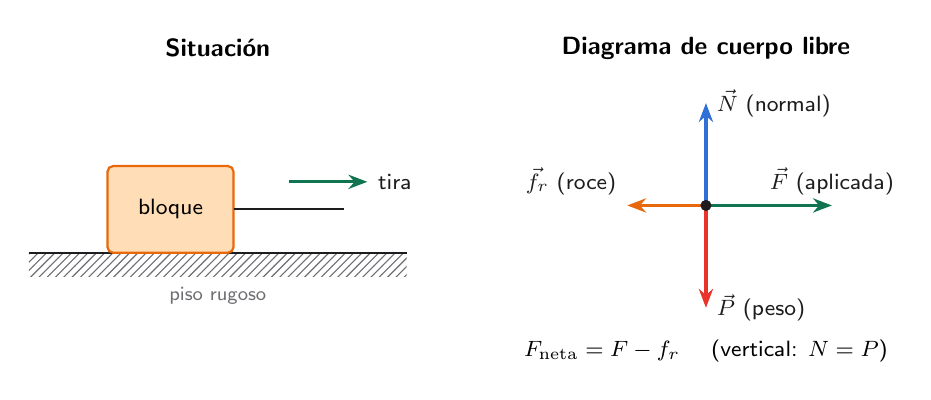
\begin{tikzpicture}[font=\footnotesize,>={Stealth[length=2.4mm]}]
% situación
\node[font=\small\bfseries] at (2,2.6) {Situación};
\fill[pattern=north east lines,pattern color=gris] (-0.4,-0.3) rectangle (4.4,0);
\draw[thick,tinta] (-0.4,0) -- (4.4,0);
\draw[thick,draw=nar,fill=narc!45,rounded corners=2pt] (0.6,0) rectangle (2.2,1.1);
\node at (1.4,0.55) {bloque};
\draw[thick,tinta] (2.2,0.55) -- (3.6,0.55);
\draw[->,very thick,menta!70!black] (2.9,0.9) -- (3.9,0.9) node[right,text=tinta] {tira};
\node[gris,font=\scriptsize] at (2,-0.55) {piso rugoso};
% diagrama de cuerpo libre
\node[font=\small\bfseries] at (8.2,2.6) {Diagrama de cuerpo libre};
\coordinate (c) at (8.2,0.6);
\draw[->,very thick,azul] (c) -- ++(0,1.3) node[right,text=tinta] {$\vec N$ (normal)};
\draw[->,very thick,coral] (c) -- ++(0,-1.3) node[right,text=tinta] {$\vec P$ (peso)};
\draw[->,very thick,menta!70!black] (c) -- ++(1.6,0) node[above,text=tinta] {$\vec F$ (aplicada)};
\draw[->,very thick,nar] (c) -- ++(-1.0,0) node[above left,text=tinta] {$\vec f_r$ (roce)};
\fill[tinta] (c) circle (2pt);
\node[font=\footnotesize] at (8.2,-1.25) {$F_{\mathrm{neta}} = F - f_r$ \quad (vertical: $N = P$)};
\end{tikzpicture}
\end{document}
